\maketitle
\newpage

\section{Геометрическая оптика}
\subsubsection*{1.15}

\begin{equation}\label{eq1} 
	\sin \alpha_{кр} = \frac{n_2}{n_1}
\end{equation}

По световоду пойдут лучи, ограниченные лучом, испытывающем на его стенке полное внутреннее отражение. На торце световода $\sin \alpha = n \sin \beta$. Из (\ref{eq1}) условие полного внутреннего отражения: $\sin (90^{\circ} - \beta) = 1/n$. Отсюда  $2\alpha = 2 \arcsin(n^2 - 1)^{1/2}$. Так будет пока $n^2 < 2$, т.е. пока $\sin \alpha < 1$. Для больших значений $n$ угловая апертура будет уже $2\alpha = \pi$.
\subsubsection*{T1}

\subsubsection*{a)}
У близорукого человека будет зрение определяться соотношением:

\begin{equation*}
	\frac{1}{L_d} + \frac{1}{b_0} = D_{бл}
\end{equation*}

Требуется, чтобы было:

\begin{equation*}
	\frac{1}{\infty} + \frac{1}{b_0} = D_{ид}. 
\end{equation*}

Таким образом требуемая сила очков будет равна:

\begin{equation*}
	\Delta D = - \frac{1}{L_d} = -2 дптр
\end{equation*}

\subsubsection*{б)}

У дальнозоркого человека оптимальное зрение определится соотношением:

\begin{equation*}
	\frac{1}{L_b} + \frac{1}{b_0} = D_{дал}
\end{equation*}

Требуется, чтобы было:

\begin{equation*}
	\frac{1}{L_0} + \frac{1}{b_0} = D_{необ}. 
\end{equation*}

Таким образом требуемая сила очков будет равна:

\begin{equation*}
	\Delta D = \frac{1}{L_0} - \frac{1}{L_b} = 3 дптр
\end{equation*}
\subsubsection*{T2}

Геометрически выходит гипербола, доказываем.

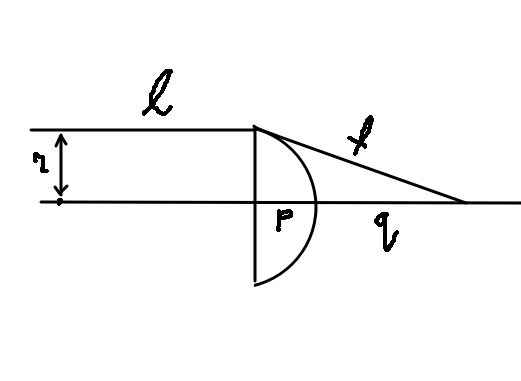
\includegraphics{parts/img/T2.png}

Так как длина оптических путей должна совпадать, то запишем равенство

\begin{equation*}
	l + f = l + np + q 
\end{equation*}

Таким образом, приходим к равенству

\begin{equation*}
	np + q = \sqrt{(p+q)^2 + r^2}
\end{equation*}

\begin{equation*}
	(n^2 - 1)p^2 + 2 p q (n -1)  = r^2
\end{equation*}
Что сводится к уравнению гиперболы в координатах $(p,r)$
\subsubsection*{1.57}

Яркость изображения в данном случае --- это освещённость получаемого изображения. Обозначая освещённость от Луны на поверхности Земли за $E_0$, для освещённости в глазу (без телескопа) получаем ,$B = E_0 \pi d_з^2 / (4S_0)$, где $S_0$ --- площадь изображения в глазу. Для увеличения в телескопе имеем

\begin{equation*}
	\Gamma = \frac{\alpha}{\beta} = \frac{f_2}{f_1}  = \frac{D}{d} 
\end{equation*}
Отношение площадей изображения в глазу $S/S_0 = (D/d)^2$.\\
Диаметр потока, выходящего из телескопа $d = D/\Gamma$ оказывается меньше диаметра зрачка лишь при $Г = 50$.\\
Пока диаметр больше --- яркость та же (случаи 1 и 2). При $\Gamma = 50$ поток (а следовательно и яркость) уменьшается в 4 раза.


\section{Формулы Френеля. Поляризация. Поток энергии и давление света}
\subsubsection*{2.1}
Ну давайте докажем, сначала разберем случай для \textbf{E}, лежащего в плоскости падения.
\begin{equation*}
	1 - R_{\|} = T_{\|} \cos{\psi} / \cos{\varphi}, \  1 + R_{\|} = nT_{\|}
\end{equation*}
\begin{equation*}
	1 - R_{\bot} = T_{\bot} \cos{\psi} / \cos{\varphi}, \  1 + R_{\bot} = nT_{\bot}
\end{equation*}

Далее выводим, что

\begin{equation*}
	1 - R_{\|}^2 = T_{\|}^2 n\cos{\psi} / \cos{\varphi} 
\end{equation*}

\begin{equation*}
	1 - R_{\bot}^2 = T_{\bot}^2 n\cos{\psi} / \cos{\varphi} 
\end{equation*}

Для потоков энергии, в случае равенства потока энергии падающей волны потокам энергии отраженной и преломлённой волн имеем

\begin{equation*}
	\cos{\varphi} E_{e\|}^2 = \cos{\varphi} E_{r\|}^2  + \cos{\psi} E_{d\|}^2 
\end{equation*}
Вводя амплитудные коэффициенты отражения и преломления находим

\begin{equation*}
	1 = R_{\|}^2 + T_{\|}^2 n\cos{\psi} / \cos{\varphi} 
\end{equation*}

Получили из формул Френеля.\\
В случае нормального падения волны ($\varphi = \psi = 0$) находим

\begin{equation*}
	1 - R_{\|} = T_{\|}, \ 1 + R_{\|} = nT_{\|}, \ 1 + R_{\bot} = T_{\bot}, \ 1 - R_{\bot} = nT_{\bot}
\end{equation*}

Отсюда получаем 
\begin{equation*}
	R_{\bot} = -R_{\|}, \  T_{\bot} = T_{\|}
\end{equation*}
ЧТД.
\subsubsection*{2.20}
\begin{equation}\label{eq2201}
	T_{\|} = 2\sin{\psi}\cos{\varphi}/ \left[\sin{(\varphi + \psi)} \cos{(\varphi - \psi)}  \right]
\end{equation}
\begin{equation}\label{eq2202}
	T_{\bot} = 2\sin{\psi}\cos{\varphi}/\sin{(\varphi + \psi)}
\end{equation}
\begin{equation}\label{eq2203}
	\Delta = (I_{\bot} - I_{\|}) / (I_{\bot} + I_{\|})
\end{equation}

Используем (\ref{eq2201}) и (\ref{eq2202}) на верхней границе, на нижней --- то же самое, но переставим $\varphi$ и $\psi$. Из \ref{eq2203}, учитывая, что падает естественный свет получим 
\begin{equation*}
	\Delta = \left[ \cos^4(\varphi - \psi) - 1 \right] / \left[ \cos^4(\varphi - \psi) + 1 \right] 
\end{equation*}
По заданным в условии величинам находим: $-0,015; \ -0,091; \ -0,176; \ -0,402$
\subsubsection*{2.27}
$E_{\|} = E_{\bot}$, $\delta = \frac{\pi}{2}$\\
\begin{equation*}
	\tg\left( \frac{\delta}{2}\right) = \frac{1-n^2}{2n} = 1
\end{equation*}
Откуда $n = 0,414$, т.е. $n_1 = 2,41$ при $n_2=1$.
%\subsubsection*{2.45}


\section{Дисперсия}
\subsubsection*{10.21}
\begin{equation}\label{eq10211}
	n^2 = \varepsilon = 1 - 4 \pi N (e^2 / m) / \omega^2 = 1 - \omega_p^2 / \omega^2 = 1 - \nu_p^2 / \nu^2
\end{equation}
\begin{equation}\label{eq10212}
	u  = c^2 / \upsilon = cn
\end{equation}
Из (\ref{eq10211}) и (\ref{eq10212}) получаем
\begin{equation*}
	u = c(1 - \omega_p^2 / \omega^2)^{1/2}
\end{equation*}
для показателя преломления близком к единице находим
\begin{equation*}
	u \approx c \left[1 - Ne^2 / (2\pi m \nu^2)\right]
\end{equation*}
Для разницы времён прихода импульсов получаем
\begin{equation*}
	\Delta t = L(1/u_1 - 1/u_2) \approx LNe^2 / (2\pi mc  \nu_1^2)
\end{equation*}
Отсюда $L = 2\pi cm \nu_1^2 \Delta t / (Ne^2) \approx 6,67 \cdot 10^{20}$ см $\approx 700$ св. лет.
\subsubsection*{10.24}
Частота ультрафиолета $\omega = E / \hbar = 5 \cdot 1,6 \cdot 10^{-12} / (1,054 \cdot 10^{-27}) \approx 8 \cdot 10^{15} c^{-1}$. Граница прозрачности определяется из (\ref{eq10211}) при $n=0$, откуда 
\begin{equation*}
	N = m \omega / (4\pi e^2) = 2 \cdot 10^{22} см^{-3}
\end{equation*}
Число атомов серебра в единице объема
\begin{equation*}
	N_{Ag} = \rho N_A / A
\end{equation*}
Получаем $N_{Ag} = 6 \cdot 10^{22} см^{-3}$
\subsubsection*{10.35}
Показатель преломления определяется соотношением
\begin{equation*}
	n = \sqrt{1 + 4 \pi \alpha N}
\end{equation*}
где $\alpha$ --- поляризуемость молекул газа (в гауссовской системе), а $N$ --- их концентрация. Принимая во внимание, что 
\begin{equation*}
	N(h) = \frac{P_0}{kT}\exp \left( -\frac{mg_Bh}{kT}\right) 
\end{equation*}
где $P_0 / kT$ --- концентрация молекул при $h = 0$, получим
\begin{equation*}
	n = \sqrt{1+ 4\pi \alpha \frac{P_0}{kT} \exp \left( -\frac{mg_Bh}{kT}\right) } \approx 1 + 2\pi \alpha \frac{P_0}{kT} \left( 1 - \frac{mg_Bh}{kT}\right) 
\end{equation*}
Радиус кривизны луча, пущенного горизонтального вблизи поверхности планеты, есть
\begin{equation*}
	r \approx - \frac{(kT)^2}{2\pi \alpha P_0 m g_B}
\end{equation*}
\begin{equation*}
	n - 1 \approx (n_0 - 1) \left[1 - mgh/(kT)\right]
\end{equation*}
Т.к. $(n-1) << 1$
\begin{equation*}
	r = -kT \left[(n_0 - 1)mg\right]
\end{equation*}
Для Земли $n_0 = 1,0003$ откуда $r \approx -2,9 \cdot 10^4 Км$. Так как радиус Земли равен $6,4 \cdot 10^3 Км$ и $n_0 -1 \sim p_0$, для круговой рефракции давление (и плотность) в атмосфере Земли должны быть увеличены в $4,5$ раза.
%\input{parts/T3}

\section{Интерференция монохроматических волн}
\subsubsection*{3.16}
\begin{equation}\label{eq3161}
	m \lambda = \Delta + \lambda / 2 = 2h(n^2 - \sin^2 \varphi)^{1/2} + \lambda / 2
\end{equation}
Получаем для угла между поверхностями пластинки $\alpha$ из (\ref{eq3161})
\begin{equation}\label{eq3162}
	\alpha = (h_{m+1} - h_m)/\Delta y = \lambda/\left[ 2 \Delta y (n^2 - \sin^2 \varphi)^{1/2}\right] 
\end{equation}
Найдем угол $\alpha$ при $n=1,5$, $\Delta y = 5мм$ и $\lambda = 5800 \buildrel _\circ \over {\mathrm{A}}$
\begin{equation*}
	\alpha = \lambda / (2n \Delta y) \approx 8''
\end{equation*}
\subsubsection*{3.11}
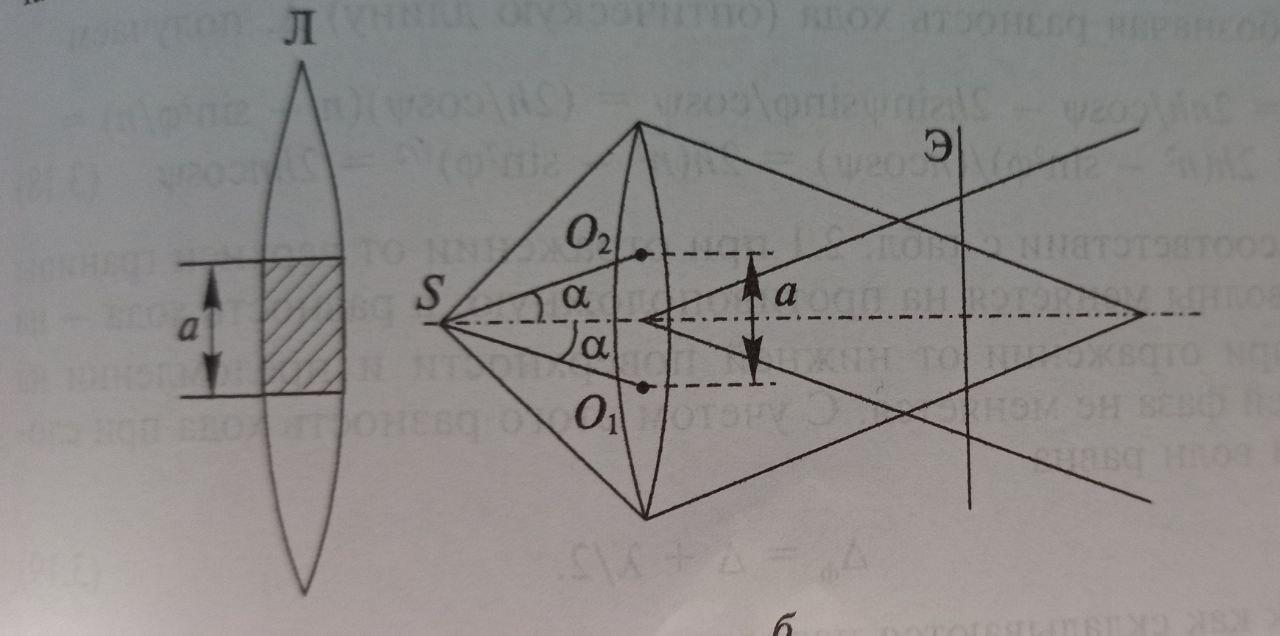
\includegraphics[width=0.4\textwidth]{parts/img/3_16.jpg}
\begin{equation*}
	\alpha = \frac{a}{f}
\end{equation*}
\begin{equation*}
	a = \frac{\lambda f}{\Delta y} = 0,6мм
\end{equation*}

\subsubsection*{3.20}
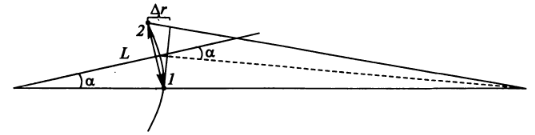
\includegraphics{parts/img/3_20.png}
На рисунке показано положение антенн (1 и 2) при повороте Земли на угол $\alpha$. Разность хода сигнала до антенн при малом угле $\alpha$ равна $\Delta r = L \sin \alpha$. Так как напряжение на контуре пропорционально квадратному корню из интенсивности, то т.к. $I = 2I_0\left[ 1 + \cos (k \Delta r)\right] $, то
\begin{equation*}
	U= U_0 \left[ \cos (k \Delta r/2)\right]  = U_0\left[ \cos(\pi L \sin \alpha / \lambda)\right]  = U_0 \cos \omega t
\end{equation*}
При малых $\alpha$ имеем $\sin \alpha \approx \alpha = \omega_з t$. Таким образом период изменения амплитуды напряжения
\begin{equation*}
	T = 2\pi / \omega = \lambda T_з / (\pi L) = 2,3 мин
\end{equation*}
\subsubsection*{3.35}
Частота лазера меняется по линейному закону $\omega = \omega_0(1 + at)$. Заменим частоту на длину волны ($\omega = 2\pi c / \lambda$), получаем $1/\lambda - 1/\lambda_0 = at/\lambda_0$. Умножая это на $L$ и учитывая, что $L/\lambda$ за период $t =T = 1/\nu$ меняется на единицу находим 
\begin{equation*}
	\nu = \frac{La}{\lambda_0} = 100 кГц.
\end{equation*}

\section{Немонохроматический свет, временная когерентность. Пространственная когерентность}
\subsubsection*{4.9}
Показатель преломления воздуха $n$ растет с увеличением плотности, которая пропорциональна давлению. При малых изменениях можно считать в данном случае для кювет длиной $l$ что $(n-1)l = a \Delta p$, где $a$ --- постоянная величина. Используя  $I = 2I_0\left[ 1 + \cos (k \Delta r)\right] $, получаем
\begin{equation*}
	 I = 2I_0( 1 + \cos  \left[ k (n-1)l\right] )
\end{equation*}
Подставляя $k = \omega / c$ и интегрируя по спектру находим 
\begin{equation*}
	I = 2(I_0/\Delta \omega) \int_{\omega_1}^{\omega_2} \left[ 1 + \cos (\omega a \Delta  p / c) \right] d\omega 	
\end{equation*}
\begin{equation*}
	I = 2I_0\left( 1 + \left[2c/(\Delta \omega a \Delta p)\right]\cos \left[(\omega_1 + \omega_2) a \Delta p /(2c)\right] \sin \left[\Delta \omega a \Delta p / (2c)\right] \right)
\end{equation*}
Обозначив $(\omega_1 + \omega_2)/2 = \omega$ получаем условие первого минимума $\omega a \Delta p_1 /c =\pi$. Картина исчезает, когда аргумент синуса становится равным $\pi = \Delta \omega a \Delta p_2 / (2c)$. Исключая $a$, находим 
\begin{equation*}
	\Delta p_2 = \Delta p_1 2 \omega/ \Delta \omega = 200 мм \ рт. \ ст.
\end{equation*}

\subsubsection*{5.13}
Для максимального порядка интерфернционных полос  при $\varphi = 0$ получаем $m_{max} = (2hn - \lambda/2)/\lambda = 1000$. Для минимального порядка при $\varphi = 90^{\circ}$ находим $m_{min} = \left[ 2h(n^2 - 1)^{1/2} - \lambda/2\right] /\lambda = 714$. Допустимую немонохроматичность оцениваем как $\Delta \lambda = \lambda/m_{max} \approx 0,56нм$. Так как зрительная труба установлена на бесконечность, картина наблюдается как бы на бесконечности, поэтому источник может быть любого размера и в любом положении.
\subsubsection*{5.13}
\begin{equation}\label{eq5131}
	D \sin \theta = m \lambda
\end{equation}
Так как плоскость наблюдения находится в зоне Фраунгофера, полуширина первого максимума определяется (\ref{eq5131}), а интенсивность следующего составляет менее $4\%$ от первого, то наблюдения возможны только в пределах области на экране $2L\lambda/b$, где $L$ --- растояние от щелей до экрана. Для монохроматического источника в схеме Юнга из $\Delta y = \lambda / (2\alpha)$ получаем ширину полос $\Delta y = \lambda L / l$ и число $N = 2l /b = 40$, поскольку это число совпадает с наблюдаемым числом $N_1$, немонохроматичность ещё не уменьшает число полосб т.е. $m_{max} = \lambda / \Delta \lambda \geq 40/2$. При уменьшении $b$ в $5$ раз число полос в отсутствии немонохроматичности должно возрасти в $5$ раз. Но этого не наблюдается. И, следовательно, ограничение связано с немонохроматичностью, т.е. $m_{max} = \lambda / \Delta \lambda = 80/2 = 40$. Откуда $\Delta \lambda = \lambda / 40 = 12,5 нм$.
%\subsubsection*{5.13}
\begin{equation}\label{eq5131}
	D \sin \theta = m \lambda
\end{equation}
Так как плоскость наблюдения находится в зоне Фраунгофера, полуширина первого максимума определяется (\ref{eq5131}), а интенсивность следующего составляет менее $4\%$ от первого, то наблюдения возможны только в пределах области на экране $2L\lambda/b$, где $L$ --- растояние от щелей до экрана. Для монохроматического источника в схеме Юнга из $\Delta y = \lambda / (2\alpha)$ получаем ширину полос $\Delta y = \lambda L / l$ и число $N = 2l /b = 40$, поскольку это число совпадает с наблюдаемым числом $N_1$, немонохроматичность ещё не уменьшает число полосб т.е. $m_{max} = \lambda / \Delta \lambda \geq 40/2$. При уменьшении $b$ в $5$ раз число полос в отсутствии немонохроматичности должно возрасти в $5$ раз. Но этого не наблюдается. И, следовательно, ограничение связано с немонохроматичностью, т.е. $m_{max} = \lambda / \Delta \lambda = 80/2 = 40$. Откуда $\Delta \lambda = \lambda / 40 = 12,5 нм$.

\section{Дифракция Френеля}
\subsubsection*{6.16}
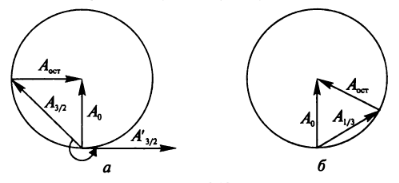
\includegraphics{parts/img/6_16.png}
На векторной диаграмме показаны амплитуды волн: в остутствие диска $A_0$, от полутора зон Френеля $A_{3/2}$, от зон вне диска $A_{ост.}$. Показатель преломления увеличивает фазу волны на $(2\pi / \lambda)(n - 1)h$. Максимум амплитуды в точке наблюдения будет, когда зона поворота $A_{3/2} = (5/4)\pi + 2\pi m $, где $m \in \mathbb{Z}^+$ (и $0$), откуда $h = (2m + 5/4)(\lambda/2)(n-1)$.
%\subsubsection*{6.31}
\begin{equation}\label{eq6311}
	r^2_m \approx 2ah_m \approx abm \lambda / (a + b)
\end{equation}
По условию фокусное расстояние $f = 1/D = 1/(2,5)\ м$. Из {\ref{eq6311}} при $a = \infty$ получаем число зон Френеля $m = r^2 / (\lambda f) = 5,5$. Интенсивность для $5,5$ зон Френеля: $I_2 = 2A_0^2$. Так как фокус линзы от всех элементов фронта, пришедшего  к отверстию, волны приходят в одинаковой фазе, все составляющие вытягиваются в прямую линию. Длина этой линии равна 5,5 полуоборотов окружности радиусом $A_0$, т.е. $A=m\pi A_0$. Интенсивность $I_1 = (m\pi)^2A_0^2$. Отношение интенсивностей $I_1/I_2 = (m\pi)^2 = 150$\\
Отношение размеров пятен можно найти из условия, что в обоих случаях в пятнах сосредоточена одна и та же энергия (проходящая через отверстие в экране) $I_1 d_1^2 = I_2 d_2^2$. Отсюда $d_1/d_2  = \sqrt{150} \approx 12$.
%\subsubsection*{6.50}
В сферической сходящейся волне наблюдается такой же эффект, как при использовании собирающей линзы: волны от всех элементов отверстия приходят в одной и той же фазе --- спираль разворачивается в прямую линию. Суммарная амплитуда соответствует длине линии. В данном случае (трёх зон) она равна $I=9 \pi^2 I_0$. Сферическая сходящаяся волна создаёт в плоскости экрана поле практически с одной амплитудой, но со сдвигом по фазе, который можно вычислить по расстоянию от фронта сферической волны до плоскости экрана. Для малых углов схождения это равно приблизительно расстоянию от точки фронта до плоскости экрана по нормали ($x$). Обозначив расстояние от оси экрана $\rho$ и считая радиус волны $\approx R_0$, получим $R_0^2 = (R_0 - x)^2 + \rho^2$, откуда $x = \rho^2/(2R_0$. Отсчитывая фазу волн от фаз волны в центре отверстия, получаем в зависимости от $\rho$ фазы волн $\phi_1 = (2\pi / \lambda)\rho^2/(2R_0)$. Аналогичным образом для точки $z$ на оси экрана находим $\phi_2 =  (2\pi / \lambda)\rho^2/(2z)$. Относительный сдвиг фаз 
\begin{equation*}
	\varphi = \varphi_2 - \varphi_1 = (\pi / \lambda) \rho^2 (1/z - 1/R_0)
\end{equation*}
Граница зон Френеля (при z $z \geq R_0$) определяется из условия $\varphi = -m\pi$. Поэтому 
\begin{equation*}
	\rho^2_m = m \lambda z R_0 / (z - R_0)
\end{equation*}
Используя условие, что при плоской волне для $R$ отверстие открывает три зоны Френеля, получаем: $D^2/4 = m \lambda z R_0 / (z - R_0) = 3 \lambda R_0$, откуда
\begin{equation*}
	m = 3(z - R_0) / z
\end{equation*}
При $z = R_0$ имеем $m = 0$. При $z  = 3R_0$ получаем $m = 2$. Две зоны Френеля дают минимум. Других минимумов нет, так как для чётных $m$ получаются отрицательные значение $z$.
%\input{parts/6_64}

\section{Дифракция Фраунгофера}
%\subsubsection*{7.10}
Для малых углов угловой радиус
\begin{equation}\label{eq7101}
	\theta_m  = [0,61 + (m - 1)/2] \lambda / R
\end{equation}
где $m = 1, 2, 3, \dots$\\
Для углового размера пятна имеем
\begin{equation}\label{eq7102}
	\theta \approx 1,22 \lambda / D
\end{equation}
Чтобы разрешать детали с размером $l$ на расстоянии $h$ необходимо $\theta \leq l/h$. Для диаметра объектива получаем $D \geq 1,22 \lambda h / l = 12 см$. Способность разрешения на плёнке связано с расстоянием между зёрнами плёнки, которое равно $1/N$. Детали изображения должны быть больше этого расстояния $(l/h) f \geq 1/N$, откуда $f \geq h / (Nl) = 40 см$. Размывания картины не будет , если отношение смещения объекта в системе, связанной с самолётом, к высоте полёта будет меньше отношения размера зерна плёнки (расстояние между штрихами) к факусному расстоянию фотоаппарата: $V \tau / h < (1/N) f$. Откуда
\begin{equation*}
	\tau < h / (N f V) \approx 0,25 \cdot 10^{-3} с
\end{equation*}
%\subsubsection*{7.53}
В соответствии с (\ref{eq7101}) находим площадь дифракционного пятна. Считая, что мощность равномерно распределяется по пятну, находим её часть, которая попадает на зрачок. Она должна быть больше той, которую видит глаз, $N \pi(d^2/4) /[(\pi/4) (L \cdot 2,24 \lambda D)^2] \geq n h \nu$. Откуда 
\begin{equation*}
	L \leq (dD/c)[N\nu /(nh)]^{1/2} \approx 3,2 \cdot 10^8 км
\end{equation*}
%\subsubsection*{7.59}
Числовая апертура $a = n \sin u$, где $u$ --- апертура из точки предмета, лежащей на оптической оси. Для повышения  числовой апертуры применяют иммерсию, т. е. жидкость с возможно высоким показателем преломления, заполняющую пространство между покровным стеклом над рассматриваемым предметом и объективом. Из \ref{eq7102} получаем 
\begin{equation*}
	\varphi = \delta / f   = 1,22 \lambda / (nD) = 1,22 \lambda / (2fn \sin u)
\end{equation*} 
Отсюда
\begin{equation*}
	\delta = 0,61 \lambda / (n \sin u)
\end{equation*}
По условию числовая апертура при $n = 1$ равна $0,9$, т. е. $\sin u = 0,9$. Поэтому в первом случае $\delta = 0,3 мкм$, а во втором $\delta = 0,19 мкм$.
%\subsubsection*{7.33}
На векторной диаграмме показаны амплитуды волн: в остутствие диска $A_0$, от полутора зон Френеля $A_{3/2}$, от зон вне диска $A_{ост.}$. Показатель преломления увеличивает фазу волны на $(2\pi / \lambda)(n - 1)h$. Максимум амплитуды в точке наблюдения будет, когда зона поворота $A_{3/2} = (5/4)\pi + 2\pi m $, где $m \in \mathbb{Z}^+$ (и $0$), откуда $h = (2m + 5/4)(\lambda/2)(n-1)$.
Так как плоскость наблюдения находится в зоне Фраунгофера, полуширина первого максимума определяется (\ref{eq5131}), а интенсивность следующего составляет менее $4\%$ от первого, то наблюдения возможны только в пределах области на экране $2L\lambda/b$, где $L$ --- растояние от щелей до экрана. Для монохроматического источника в схеме Юнга из $\Delta y = \lambda / (2\alpha)$ получаем ширину полос $\Delta y = \lambda L / l$ и число $N = 2l /b = 40$, поскольку это число совпадает с наблюдаемым числом $N_1$, немонохроматичность ещё не уменьшает число полосб т.е. $m_{max} = \lambda / \Delta \lambda \geq 40/2$. При уменьшении $b$ в $5$ раз число полос в отсутствии немонохроматичности должно возрасти в $5$ раз. Но этого не наблюдается. И, следовательно, ограничение связано с немонохроматичностью, т.е. $m_{max} = \lambda / \Delta \lambda = 80/2 = 40$. Откуда $\Delta \lambda = \lambda / 40 = 12,5 нм$.

\section{Спектральные приборы}
%\subsubsection*{8.37}
Чтобы полностью использовать разрешающую способность рещётки, надо несильно испортить остроту максимумов, которыми определяется способность к разрешению, т. е. должно выполняться условие: $b/f << \theta \approx \lambda / (Nd)$, отсюда $b < f \lambda / (Nd) \approx 0,001 см$.
%\subsubsection*{8.47}
\begin{equation}\label{eq8471}
	R = \lambda / d \lambda = mN
\end{equation}
Используя (\ref{eq8471}), для разрешающей способности решетки получаем
\begin{equation*}
	R = \lambda / \delta \lambda = \nu / \delta \nu =  c / (\lambda \delta \nu) = c \tau / \lambda = mN = m L / d = m L n
\end{equation*}
Откуда $L = c \tau / (\lambda m n) = 100см$.
%\input{parts/T5}
%\input{parts/T6}

